% !TeX spellcheck = en_GB
\documentclass[11pt]{article}

\usepackage[type1]{libertine}
\usepackage[a4paper,top=35mm]{geometry}
\usepackage{parskip}
\usepackage{amsmath, amsthm, amssymb} 
\usepackage{booktabs}
\usepackage{tabularx}
\usepackage[english]{babel}
\usepackage{enumitem}	% remove inline if not needed
\usepackage{gensymb}
\usepackage{bm}
\usepackage{graphicx}
\usepackage{xcolor}
\usepackage{float}
\usepackage{wrapfig}
\usepackage[makeroom]{cancel}
\usepackage{multicol}
\usepackage{multirow}
\usepackage{vwcol} 	 	% Provides variable multicol
\usepackage{commath} 	% Provides good differentials
\usepackage{esint} 		% Provides various fancy integral symbols
\usepackage{siunitx} 	% Provides good units
\usepackage{nicefrac}
\usepackage{dashrule}
%\usepackage{showframe}

\usepackage[titletoc,title,toc,page]{appendix}

\usepackage{hyperref}
\hypersetup{
	pdftitle={Tutorial 8 (Oscillations) Suggested Worked Solutions},
	pdfauthor={Sun Yudong},
	bookmarksnumbered=true,
	bookmarksopen=true,
	bookmarksopenlevel=2,
	pdfstartview=Fit,
	pdfpagemode=UseOutlines,
	colorlinks=true,
	linkcolor=black,
	filecolor=magenta,      
	urlcolor=blue
}
\urlstyle{same}

% custom environments
\usepackage{tikz}
\newcommand*\circled[1]{\tikz[baseline=(char.base)]{
		\node[shape=circle,draw,inner sep=2pt] (char) {#1};}}

\newcommand{\uvec}[1]{\boldsymbol{\hat{\textbf{#1}}}}
\newcommand{\bvec}[1]{\boldsymbol{\vec{#1}}}
\def\doubleunderline#1{\underline{\underline{#1}}}
\newcommand{\solution}[1]{\textbf{Solution: } #1 \hspace{5mm}}
\newcommand{\calc}{\boxed{\textbf{CALC}} \hspace{1em}}


\renewcommand{\ttdefault}{cmtt}
\newlength{\currentparskip}

\newenvironment{multicolFigure}
{\par\medskip\noindent\minipage{\linewidth}}
{\endminipage\par\medskip}

\title{Tutorial 8 (Oscillations)\\Suggested Worked Solutions}
\author{Sun Yudong}
%\date{June 10, 2018}

\begin{document}
	\maketitle
	The following only contains the worked solutions to discussion questions in Tutorial 8 (Oscillations).
	
	For Self-Review questions, please refer to the other uploaded document.
	
	\begin{enumerate}[label={[D\arabic*]},itemsep={1em}]
		\item 
			\begin{enumerate}[label={(\roman*)}]
				\item \solution{Yes} As it is perfectly elastic, the ball will bounce to the same height every time. The ball then repeats its motion after every bounce, making the motion a periodic one. 
				\item \solution{No}
				Acceleration experienced by the ball is constant, equals $g$.
			\end{enumerate}
		\item \solution{\SI{0.17}{\second}}
			
			We often use the approximation of $\left(\sin\theta \approx \theta\right)$ and subsequently the derived $T = 2\pi\sqrt{\nicefrac{l}{g}}$ to find the period of a pendulum. But from \url{arxiv.org/pdf/physics/0510206.pdf}, we find that this approximation requires that the \textbf{amplitude of the displaced angle be less than \SI{7}{\degree} for an error of less than 0.1\%} (the typical experimental error obtained with a stopwatch). 
			
			You may use the methods described in that paper, or \url{dx.doi.org/10.1088/0143-0807/29/5/021} to find that the maximum angle of displacement is \SI{2.88}{\degree} which is safely below the \SI{7}{\degree} limit. I shall skip the steps here as it is rather long and complicated. 
			
			So it is pretty safe to assume that the pendulum moves with a simple harmonic motion.
			
			Or you can ignore the previous few paragraphs and straight out assume that the motion of the pendulum is harmonic. 
			
			From \SI{650}{\milli\meter} to \SI{675}{\milli\meter}, the pendulum has moved from the equilibrium point to halfway between the equilibrium and the maximum amplitude:
			
			\begin{figure}[ht!]
				%\vspace{-0.7cm}
				\centering
				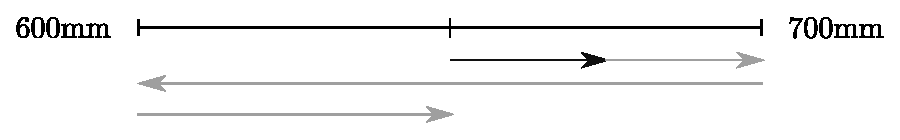
\includegraphics[width=10cm]{D2.eps}
				\vspace{-0.7em}
			\end{figure}
			
			Thus,
			\begin{align*}
				\frac{1}{2}\cancel{A_0} &= \cancel{A_0} \sin\left(\omega t\right) \\
				t &= \frac{\arcsin\left(0.5\right)}{\omega} = \frac{T\arcsin\left(0.5\right)}{2\pi} = \frac{1}{6}~\si{\second} = \doubleunderline{\SI{0.17}{\second}}
			\end{align*}
		
		\item \solution{B}
		
			The tension of the spring is the elastic force, which is proportional to the displacement $x$. Thus, the graph must be a straight line. 
			
			Alternatively, we can see that the tension $T-mg$ is proportional to the acceleration of the mass. Since the mass is oscillating, its acceleration must be proportional to the displacement $x$ from the equilibrium position, Thus, the graph must be a straight line.
			
			Since the mass has zero acceleration, and thus no net force, at the equilibrium point $x = 0$, tension $T$ at $x = 0$ must be $mg$.
		
		\item \solution{C}
			\begin{center}
				\begin{tabular}{lll}
					\toprule
					Point & Acceleration & Velocity \\
					\midrule
					A & Zero & Down\\
					B & Up & Zero\\
					\textbf{C} & \textbf{Down} & \textbf{Up}\\
					D & Down & Down\\
					\bottomrule
				\end{tabular}
			\end{center}
		
		\item \solution{\SI{2}{\hour}}
			Shifitng the entire graph \SI{2}{\meter} down:
			\begin{align*}
				\omega = \frac{2\pi}{T} = \frac{2\pi}{12} = \frac{\pi}{6} \implies x &= -\cos\left(\frac{\pi}{6}~t\right) \\
				1.5 - 2 &= -\cos\left(\frac{\pi}{6}~t\right) && \text{when the tide is at \SI{1.5}{\meter}} \\
				0.5 &=  \cos\left(\frac{\pi}{6}~t\right) \\
				t &= \frac{\cancel{\pi}}{3} \times \frac{6}{\cancel{\pi}} \\
				&= \doubleunderline{\SI{2}{\hour}}
			\end{align*}
		
		\item 
			\begin{enumerate}[start=2]
				\item 
					\begin{enumerate}[label={(\roman*)}]
						\item \textcolor{white}{.}
							\begin{figure}[ht!]
								\vspace{-0.7cm}
								\centering
								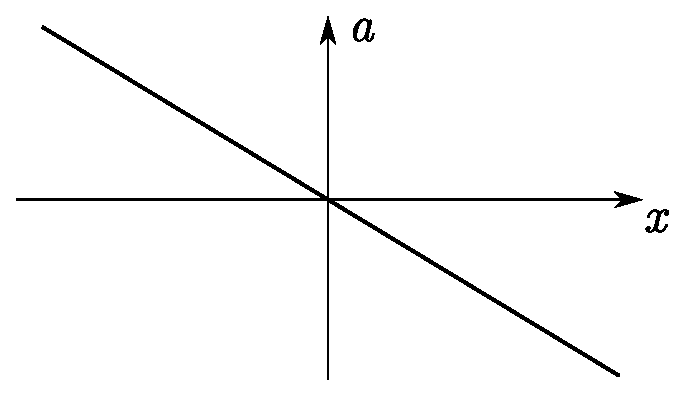
\includegraphics[width=5cm]{D6.eps}
							\end{figure}
						\item 
							\begin{enumerate}[label={\arabic*.}]
								\item $\omega = 2\pi\! f = \doubleunderline{26\pi}$ 
								\item $9.81 = \left(26\pi\right)^2 x_0 \implies x_0 = \doubleunderline{\SI{1.47e-3}{\meter}}$
							\end{enumerate}
					\end{enumerate}
				\item When the acceleration of the oscillator exceeds that of gravity, there wouldn't be any force to provide the sand with this acceleration. Thus, the fastest the sand can acceleration will be $g$, and the sand will leave the surface of the plate when the oscillator is on its way down. 
			\end{enumerate}
		
		\item \solution{D}
			\begin{equation*}
				\text{TE} = \frac{1}{2}m\omega^2x_0^2 = \frac{1}{2}m\left(\frac{2\pi}{T}\right)^2a^2 = \doubleunderline{\frac{2m\pi^2a^2}{T^2}}
			\end{equation*}
			
		\item \solution{\SI{1.8}{\second}}
			
			Using the equation derived in the previous question:
			\begin{align*}
				U = \frac{2\pi^2mx_0^2}{T^2} \implies T &= \sqrt{\frac{2\pi^2mx_0^2}{U}} \\
				&= \sqrt{\frac{2\pi^2\left(4\right)\left(0.2\right)^2}{1.0}} = \doubleunderline{\SI{1.8}{\second}}
			\end{align*}
		
		\item 
			\begin{enumerate}
				\item 
					\begin{enumerate}
						\item 
							\begin{itemize}
								\item The graph shows that $a$ is directly proportional to $x$.
								\item Since the graph is a downward slope, we deduce that the acceleration is in the opposite direction $x$:
									\begin{equation*}
										a \propto -x
									\end{equation*}
							\end{itemize} 
							\vspace{-0.5em}
							Since these are the defining features of a simple harmonic motion, the motion of the particle P is simple harmonic.
						\item \solution{\SI{460}{\hertz}}
							\begin{align*}
								\text{Gradient} = -\omega^2 = \frac{3400 - 0}{\left(\left(-0.40\right)-0.00\right)\times 10^{-3}} &= -2\pi\! f \\
								f &= \frac{\sqrt{8.5\times 10^6}}{2\pi} = \doubleunderline{\SI{460}{\hertz}}
							\end{align*}
					\end{enumerate}
				\item 
					\begin{enumerate}
						\item 
							The area under the graph from $x=0$ to $x=-0.4$ is the maximum work done per unit mass of the restoring force on the oscillating mass. Given that the graph has the equation $a = -Gx$:
							\begin{equation*}
								\phi_\text{max} = \frac{1}{2}\times A \times G\!A = \frac{1}{2}G\!A^2
							\end{equation*}
							where $A = \num{0.4e-3}$.
							
							Thus, the maximum kinetic energy $E_\text{max}$ is given by:
							\begin{equation*}
								E_\text{max} = m\phi = \doubleunderline{\frac{1}{2}mG\!A^2}
							\end{equation*}
						\item \solution{\SI{1700}{\joule}}
							\begin{align*}
								E_\text{max} &= \frac{1}{2}mG\!A^2 \\
								&= \frac{1}{2}\left(\num{2.5e-3}\right)\left(8.5\times 10^6\right)\left(\num{0.4e-3}\right)^2 = \SI{1.7}{\milli\joule}
							\end{align*}
					\end{enumerate}
			\end{enumerate}
		
		\item 
			\begin{enumerate}
				\item
					\hspace{0.5em}
					\begin{tabular}{ll}
						\toprule
						Frequency			& Time taken per oscillation \\
						Angular Frequency	& Rate of the change of phase angle per unit time \\
						\bottomrule
					\end{tabular}
					\vspace{0.5em}
				\vfill
				\item 
					\begin{enumerate}
						\item 
							\begin{equation*}
								\Delta\text{GPE} = mgh = 0.4\times 0.2 \times 9.81 = \doubleunderline{\SI{0.785}{\joule}}
							\end{equation*}
						\item 
						
							At equilibrium:
							\begin{equation*}
								kx = mg \implies k = \frac{mg}{x}
							\end{equation*}
							Thus, the change EPE is:
							\begin{equation*}
								\Delta\text{EPE} = \frac{1}{2}kx^2 = \frac{mgx}{2} =  \frac{1}{2} \times 0.4\times 0.2 \times 9.81 = \doubleunderline{\SI{0.392}{\joule}}
							\end{equation*}
					\end{enumerate}
				\vfill
				\item 
					Energy is lost as heat (and sound). \textit{This is similar to critical damping.}
					
					In the undisturbed case where you let the mass drop \textit{without providing a force to gently lower it down}, $mg > kx$, causing the mass to accelerate as GPE is converted into KE and EPE. At the point where $mg = kx$, the mass experiences no acceleration, and continues going until at some point, all the GPE is converted into KE and EPE, and all the KE is also converted into EPE ($v=0$). 
					
					Essentially, the mass will oscillate; and at the equilibrium point where $mg = kx$, the velocity of the mass is non-zero.
					
					Now, for the case in which we \textit{gently} lower it down, we are making sure that at the equilibrium point (where $mg = kx$), the velocity is zero instead of the usual non-zero. This means that we are doing work to the system by slowing it down, causing energy to be dissipated as heat (and sound).
					
					%At this point you might also realize that $\Delta \text{GPE} = \frac{1}{2} \Delta \text{EPE}$. This makes sense intuitively; oscillations are symmetrical in nature and so the conversion of energy should also be symmetrical about the equilibrium point (where $mg = kx$), thus resulting in the nice \nicefrac{1}{2}.
				\vfill
				\item \textit{For the following parts, you can also make use of the fact that $\omega = \sqrt{\nicefrac{k}{m}}$ for a spring mass system.} Let $x_1$ be the extension of the spring at equilibrium.
					\begin{enumerate}
						\item \textcolor{white}{.}
							\vspace{-1.7\baselineskip}
							\begin{align*}
								\text{Resultant Force} = kx - mg &= \left(\frac{mg}{x_1}\right)x_\text{max} - mg \\
								&= mg\left(\frac{x_\text{max}}{x_1} - 1\right) \\
								&= \left(0.400\right)\left(9.81\right)\left[\frac{0.200 + 0.200}{0.200} - 1\right] \\
								&= \doubleunderline{\SI{3.92}{\newton}~\text{upwards}}
							\end{align*}
						\pagebreak[1]
						\item \textcolor{white}{.}
							\vspace{-2\baselineskip}
							\begin{align*}
								F_\text{max} = ma_\text{max} = m\omega^2x_0 &= mg\left(\frac{x_\text{max}}{x_1} - 1\right) \\
								\omega &= \sqrt{\frac{g\left(x_\text{max}/x_1-1\right)}{x_0}} \\
								&= \doubleunderline{\SI{7.00}{\radian\per\second}}
							\end{align*}
						\item \textcolor{white}{.}
							\vspace{-1.8\baselineskip}
							\begin{align*}
								v_\text{max} = \omega x_\text{0} &= \sqrt{\frac{g\left(x_\text{max}/x_1-1\right)}{x_0}} \times x_\text{0} \\
								&= \doubleunderline{\SI{1.40}{\meter\per\second}}
							\end{align*}
					\end{enumerate}
				\item \textcolor{white}{.}
					\begin{figure}[ht!]
						\vspace{-0.7cm}
						\hspace{2cm}
						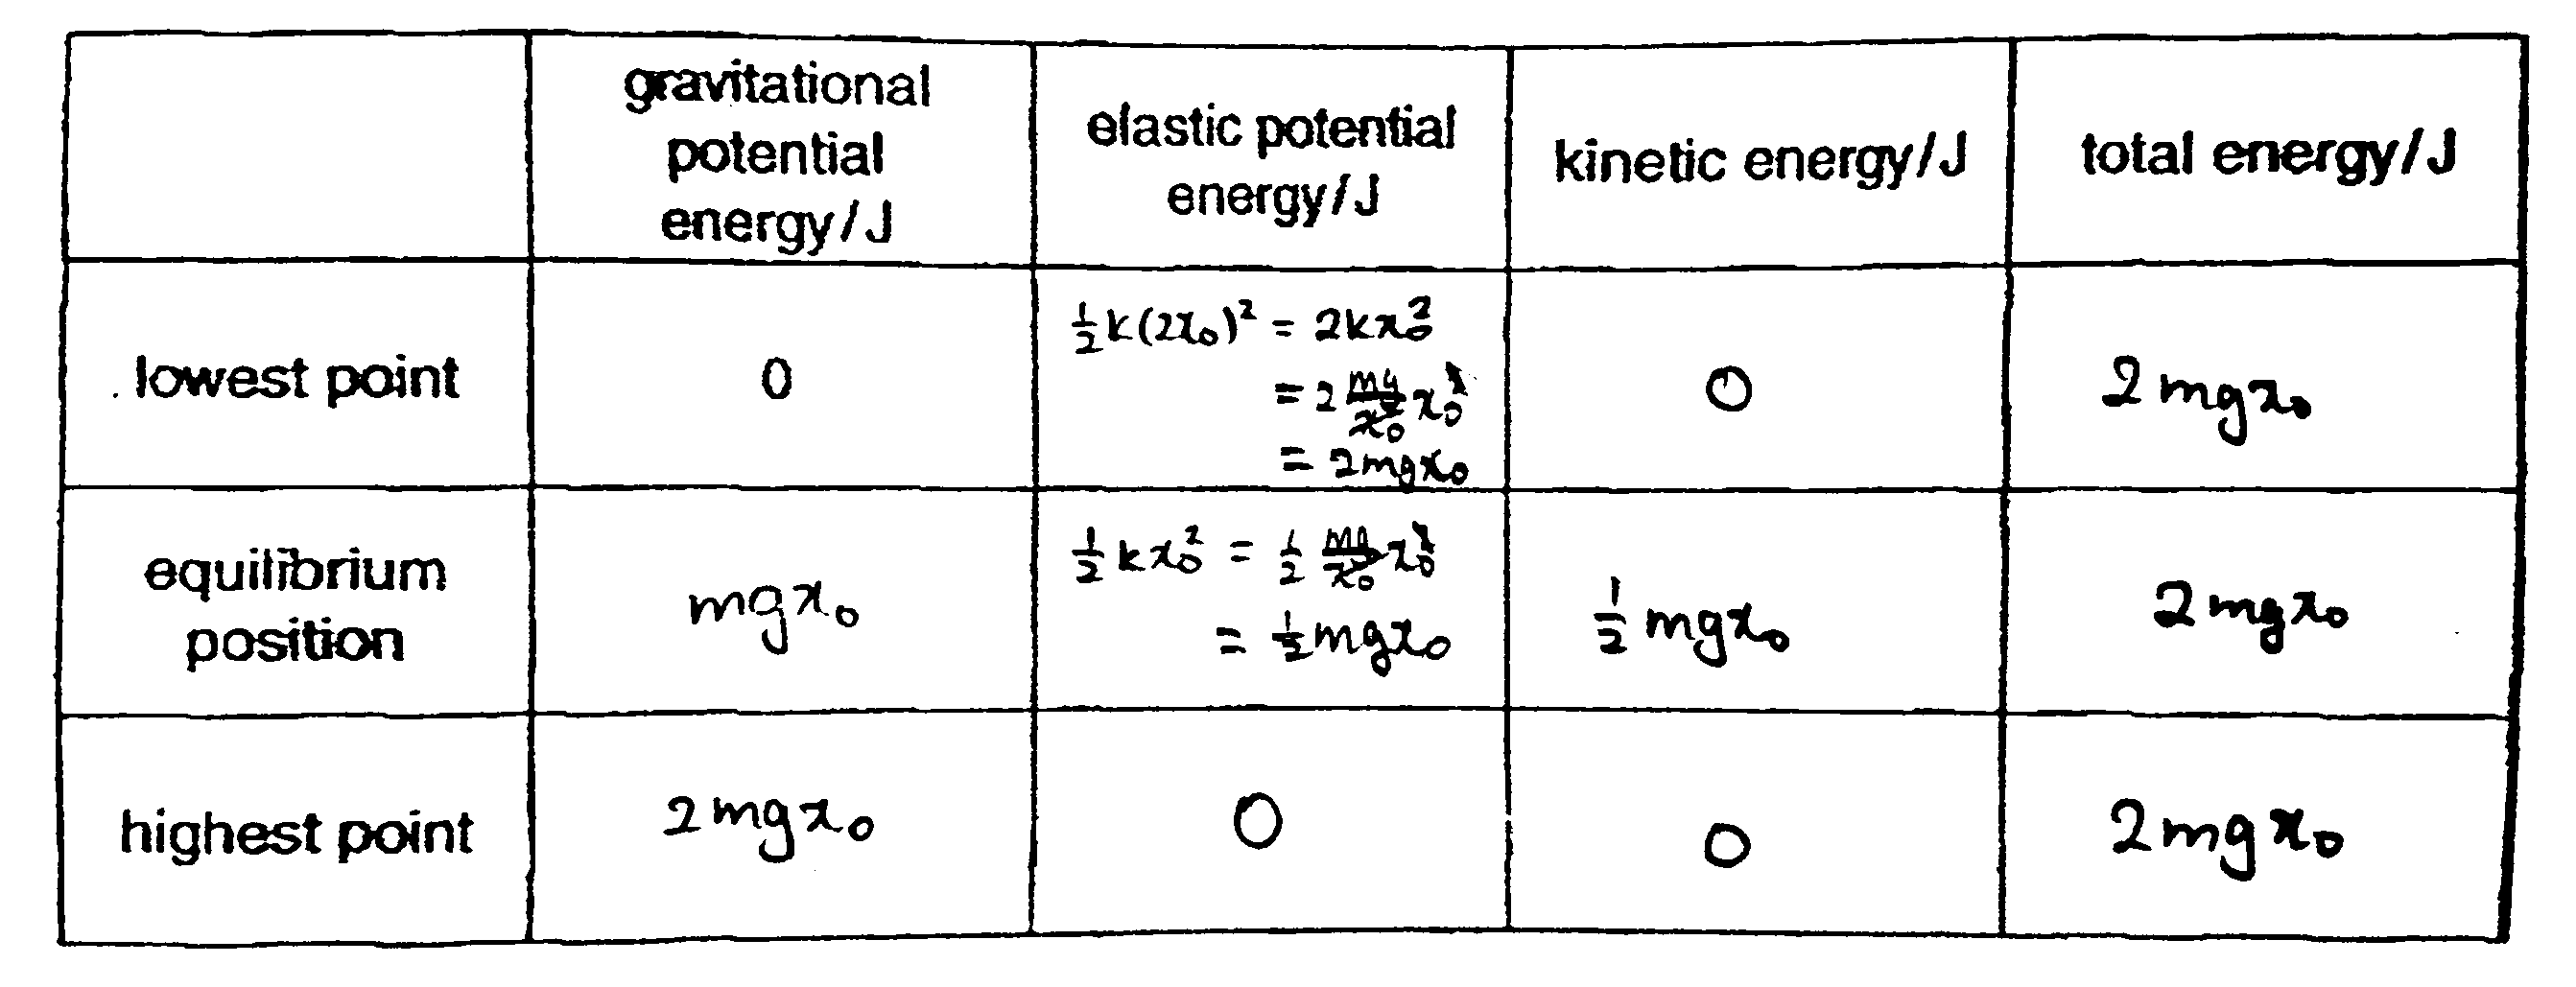
\includegraphics[width=12cm]{D10e.png}
					\end{figure}
				\item \textcolor{white}{.}
					\begin{figure}[ht!]
						\vspace{-0.7cm}
						\hspace{2cm}
						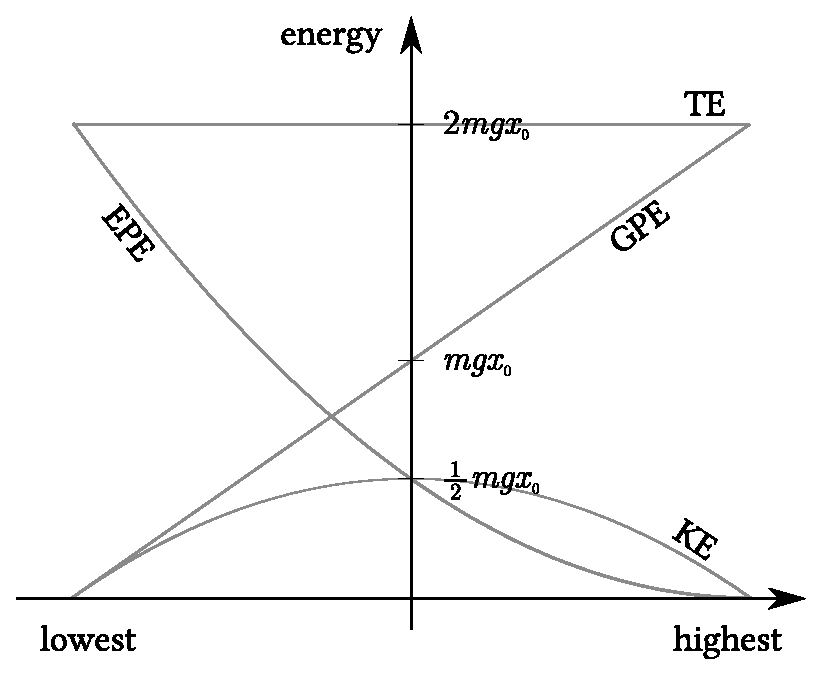
\includegraphics[width=8cm]{D10f.eps}
					\end{figure}
			\end{enumerate}
		\item
			\begin{enumerate}
				\item Upthurst is the result of the difference in fluid pressure between the top and bottom of a partially or fully submerged object. Its magnitude is equal to the weight of the fluid displaced. 
				\item Since the tube is floating in the liquid, $U = mg$:
					\begin{equation*}
						\rho V_\text{displaced} \cancel{g} = m\cancel{g} \implies m = \rho Ah
					\end{equation*}
				\item 
					\begin{enumerate}
						\item The acceleration $a$ is proportional to the displacement $x$, and points in the opposite direction of $x$.
						\item \textcolor{white}{.}
							\vspace{-1.5\baselineskip}
							\begin{align*}
								\omega^2 = \left(\frac{\rho Ag}{m}\right) \implies 2\pi\!f &= \sqrt{\frac{\rho Ag}{m}} \\
								f &= \sqrt{\frac{\rho Ag}{4\pi^2m}} \\
								&= \sqrt{\frac{\left(\num{1.0e3}\right)\left(\num{4.2e-4}\right)\left(9.81\right)}{4\pi^2\left(\num{32e-3}\right)}} = \doubleunderline{\SI{1.8}{\hertz}}
							\end{align*}
					\end{enumerate}
				\item 
					\begin{enumerate}[label={(\roman*)}]
						\item 
							\begin{enumerate}[label={\arabic*.}]
								\item 
									Time taken for 3 full oscillations $= \SI{1.5000}{\second}$. \\
									Thus, $f = 1/T = 1/(1.5000/3) = \SI{2.0}{\hertz}$
									
									\textit{\small Note; When reading off graphs, you can be precise up to half of the smallest square. e.g. the precision of the given graph $= 0.25/20 = 0.0125 \implies$ up to 4 decimal places, but the last decimal place is either 5 or 0.}
								\item \textcolor{white}{.}
									\vspace{-\baselineskip}
									\begin{equation*}
										\omega^2 = \left(2\pi\!f\right)^2 = \frac{\rho Ag}{m} \implies \rho = \frac{m\left(2\pi\!f\right)^2}{Ag} = \doubleunderline{\SI{1.2e3}{\kilogram\per\meter\cubed}}
									\end{equation*}
							\end{enumerate}
						\item 
						\begin{enumerate}[label={\arabic*.}]
							\item 
								\begin{itemize}
									\item Resistive forces due to the viscosity of the liquid. 
									\item Energy is brought away from the oscillating tube as waves in the fluid.
								\end{itemize}
							\item \textcolor{white}{.}
								\vspace{-1.5\baselineskip}
								\begin{align*}
									A_{t = 0.0} &= \SI{1.50}{\centi\meter}; A_{t = 1.0} = \SI{0.85}{\centi\meter} \\
									\implies \Delta E &= \frac{1}{2}m\omega^2\left(A_{t = 0.0}^2 - A_{t = 1.0}^2\right) \\
									&= \frac{1}{2}\left(\num{32e-3}\right)\left(2\pi\times 2.0\right)^2\left[\left(\SI{1.50e-2}{}\right)^2-\left(\SI{0.85e-2}{}\right)^2\right] \\
									&= \doubleunderline{\SI{3.86e-4}{\joule}}
								\end{align*}
						\end{enumerate}
					\end{enumerate}
			\end{enumerate}
		\item It is important so that all the sounds produced will be at the correct volume, and not a volume amplified due to resonance of the diaphragm cone...etc.
		\item 
			\begin{enumerate}
				\item 
					\begin{enumerate}[label={(\roman*)}]
						\item A forced oscillation is one that is under the influence of/driven by an external periodic force. 
						\item The effect illustrated is that of \textit{resonance}.
					\end{enumerate}
				\vspace{1.5em}
				\item 
					\begin{enumerate}[label={(\roman*)}]
						\item Form the graph, $x_{0_\text{max}} = \SI{1.600e-2}{\meter}$ and $f_\text{max} = \SI{12.0}{\hertz}$:
							\begin{enumerate}[label={\arabic*.}]
								\item $v_\text{max} = \omega x_0 = 2\pi\!f_\text{max}x_{0_\text{max}} = \doubleunderline{\SI{1.21}{\meter\per\second}}$
								\item $a_\text{max} = \omega^2 x_0 = \left(2\pi\!f_\text{max}\right)^2\!x_{0_\text{max}} = \doubleunderline{\SI{91.0}{\meter\per\second\squared}}$
							\end{enumerate}
						\item Time interval $=\frac{1}{4}T = \frac{1}{4f_\text{max}} = \doubleunderline{\SI{0.0208}{\second}}$
					\end{enumerate}
				\vspace{1.5em}
				\item \textcolor{white}{.}
				
					\vspace{-1.7\baselineskip}
					{	
						\renewcommand{\arraystretch}{1.5}
						\begin{tabular}{p{8cm}r@{}}
							With an increased mass, the acceleration experienced by the machine at every frequency is reduced. ($F = ma$) This is similar to increasing the damping of the machine.
							&
							\multirow{2}{*}{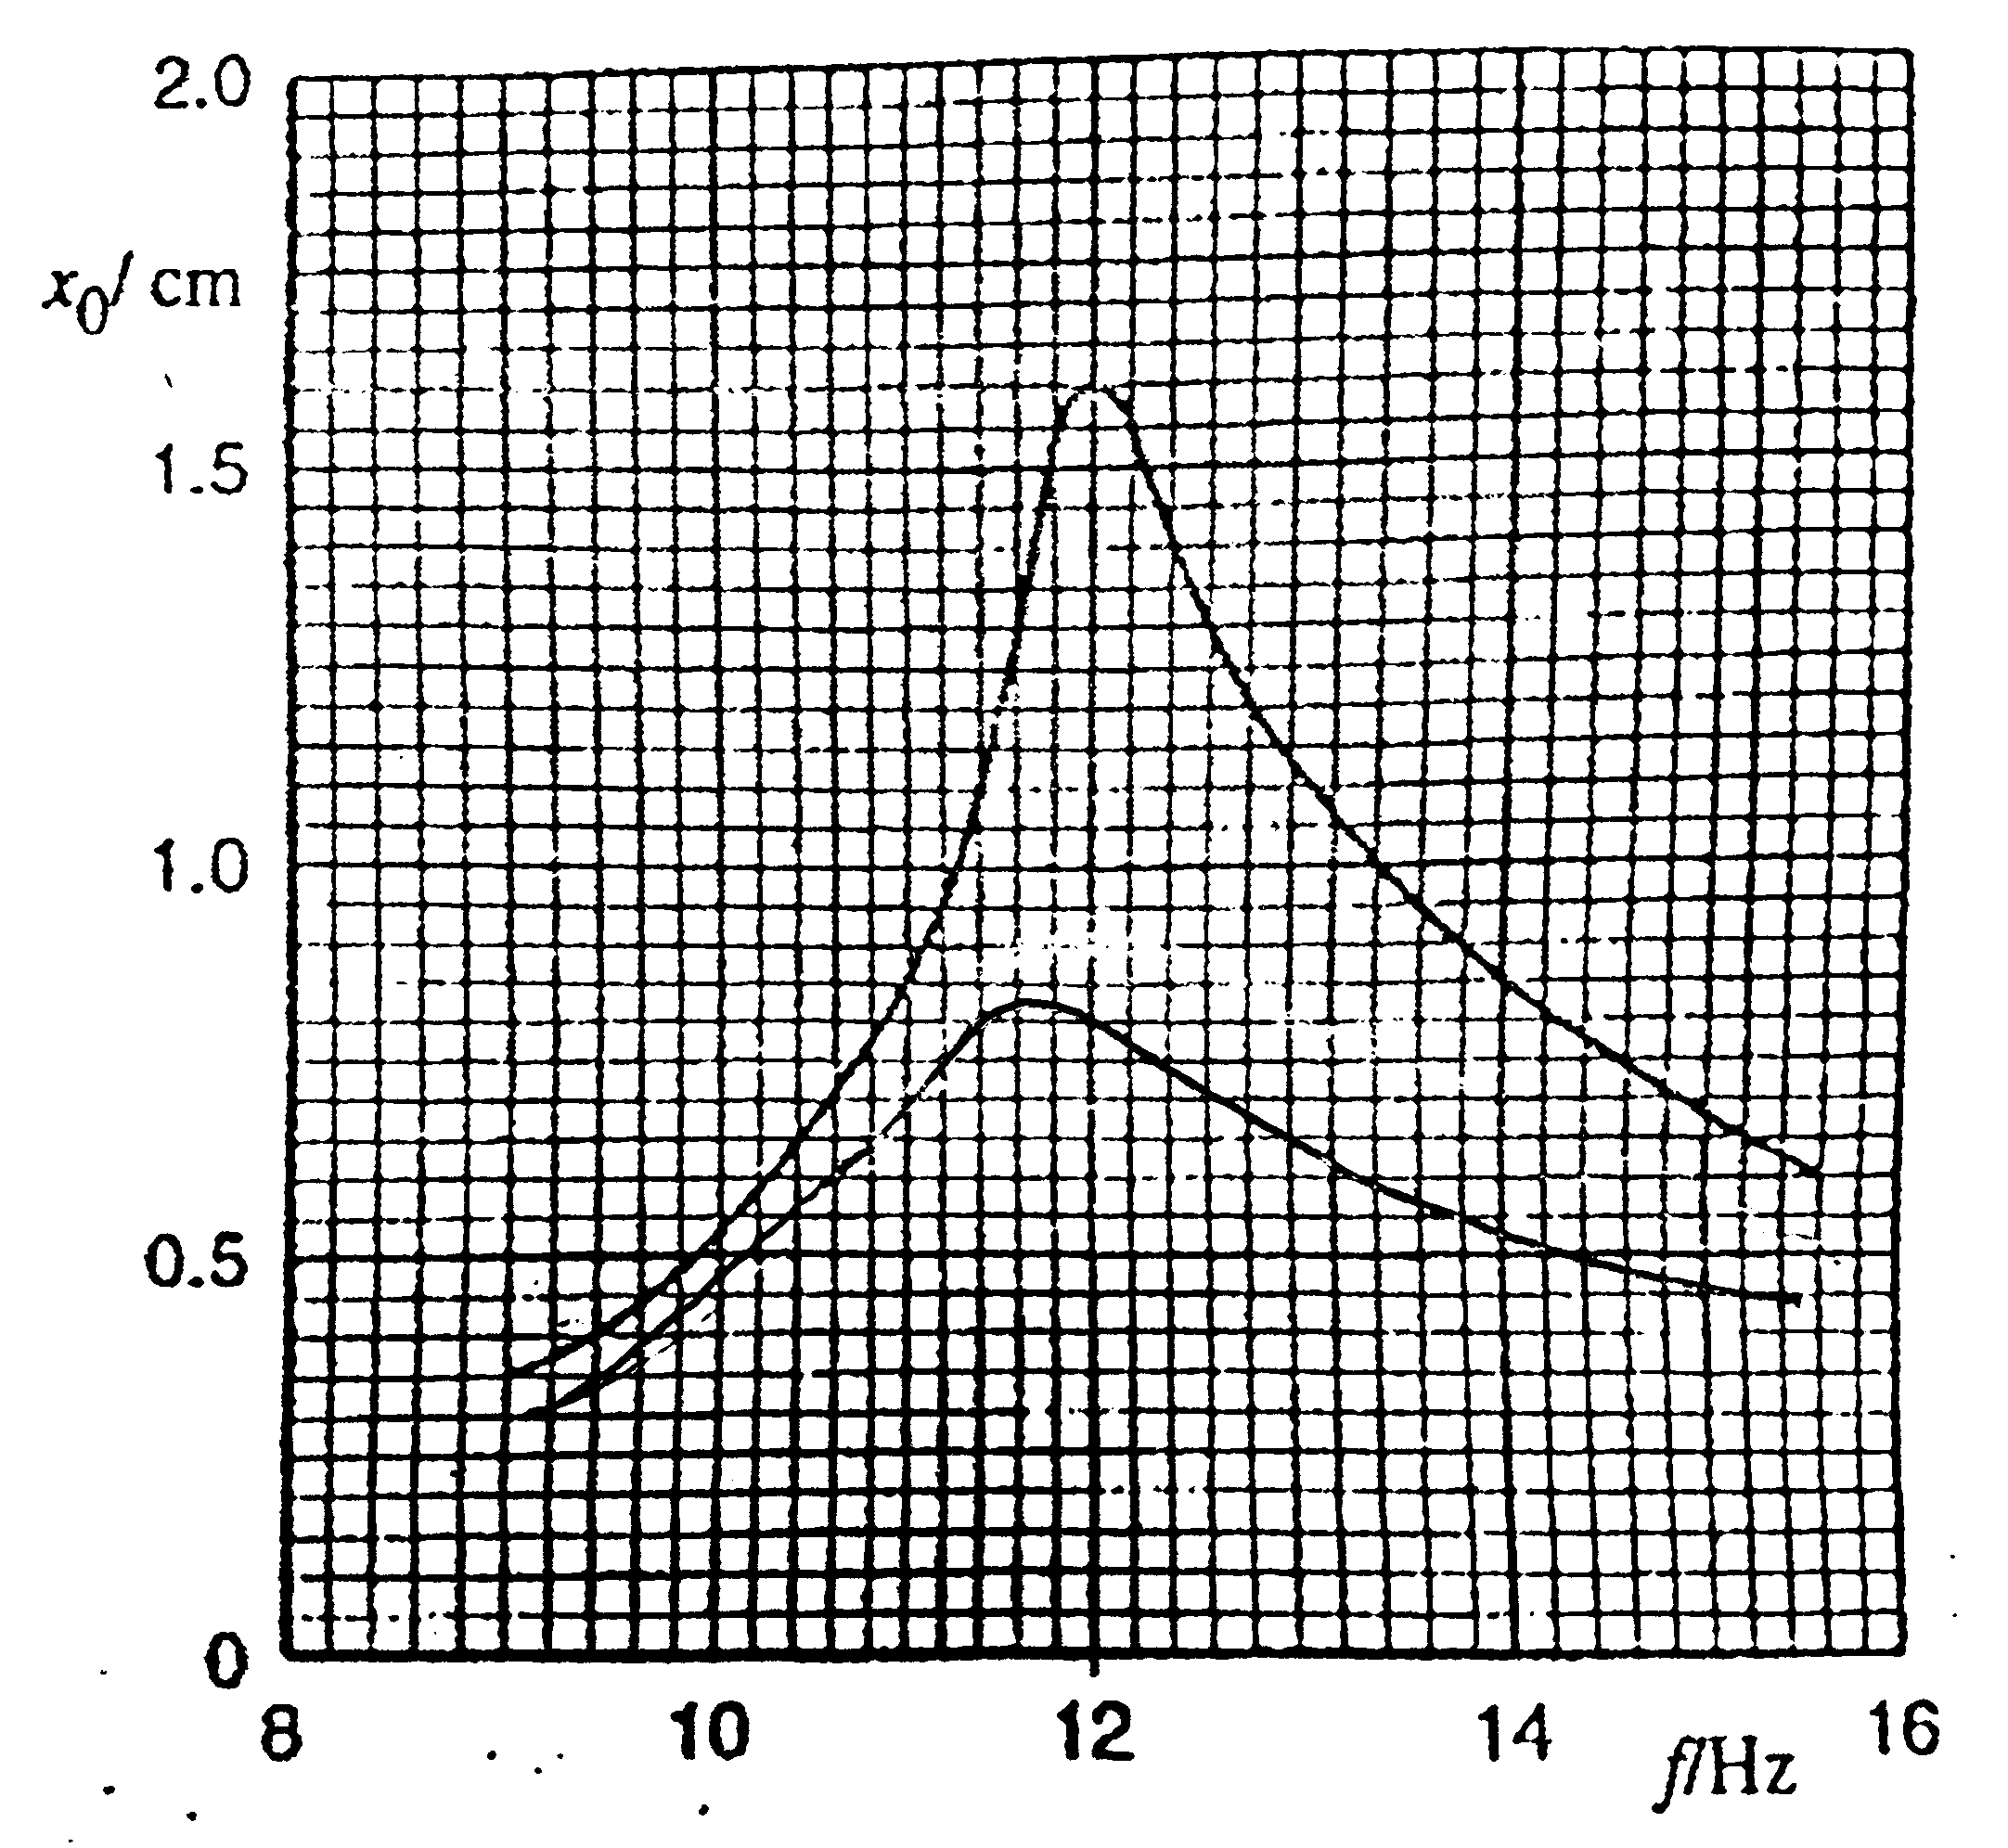
\includegraphics[height=5cm]{D13c.png}}\\
							
							The new graph would:
							\begin{itemize}
								\item have a lower maxima than the original
								\item have $f_{\text{max}_1} < f_{\text{max}_0}$
								\item not intersect the original graph
							\end{itemize}
						\end{tabular}
					}
			\end{enumerate}
		\pagebreak[4]
		\item
			\begin{enumerate}
				\item The force experienced by an object is the rate of change its linear momentum.
				\item 
					\begin{enumerate}[label={(\roman*)}]
						\item \textcolor{white}{.}
							\begin{figure}[ht!]
								\vspace{-0.7cm}
								\centering
								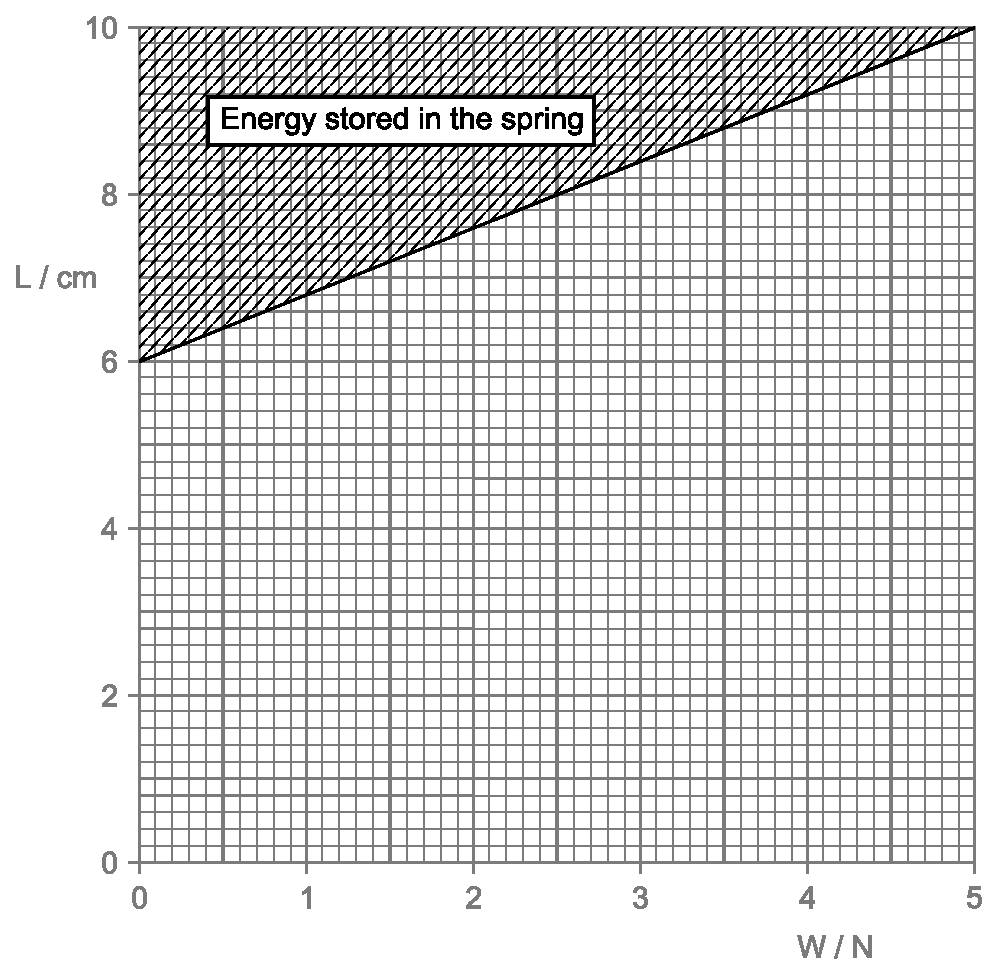
\includegraphics[width=10cm]{D14bi.eps}
								\vspace{-0.4cm}
							\end{figure}
						\item To find the energy stored in the spring $E$, we simply find the area of the shaded triangle in the previous part. 
						
						Since at every point on the graph, the spring/mass system is in a static equilibrium, the elastic force $F_S$ must be equal to the weigh $W$. Hence, we see that the base of the triangle is $kx$.
						
						The height is naturally just the extension $x$, since at \SI{6}{\centi\meter}, there isn't any weight on the spring and the spring is at its natural unstretched length. 
						
						Thus,
						\begin{equation*}
							E = \frac{1}{2}\left(kx\right)\left(x\right) = \doubleunderline{\frac{1}{2}kx^2}
						\end{equation*}
					\end{enumerate}
				\item 
					\begin{enumerate}[label={(\roman*)}]
						\item 
							Reading off the graph, when $W=\SI{4.0}{\newton}$, $L = \SI{9.2}{\centi\meter}$. Since it is then pulled downwards a distance \SI{0.80}{\centi\meter}, the total length of the spring is:$$\SI{9.2}{\centi\meter} + \SI{0.80}{\centi\meter} = \doubleunderline{\SI{0.10}{\meter}}$$
						\item 
							\begin{enumerate}[label={\arabic*.}]
								\item $\Delta \text{GPE} = mg\Delta h = W\!\Delta h =  \doubleunderline{\SI{-0.032}{\joule}}$
								\item Since $k$ is given by the negative inverse gradient of the graph:
								\begin{align*}
									\Delta \text{EPE} &= \frac{1}{2}k\left(x_{\!f}^2 - x_i^2\right) \\[0.3em]
									&= \frac{1}{2}\left[\frac{5}{\num{4.0e-2}}\right]\left[\left(\num{4.0e-2}\right)^2 - \left(\num{3.2e-2}\right)^2\right] \\
									&= \doubleunderline{+\SI{0.036}{\joule}}
								\end{align*}
							\end{enumerate}
						\item \textcolor{white}{.}
							\vspace{-2.2em}
							\begin{flalign*}
								\text{Work Done} &= \Delta \text{GPE} + \Delta \text{EPE} &\\
								&= -0.032 + 0.036 = \doubleunderline{\SI{4.0e-3}{\joule}} &
							\end{flalign*}
					\end{enumerate}
				\item 
					\begin{enumerate}[label={(\roman*)}]
						\item Total Energy $=$ Work Done $= \doubleunderline{\SI{4.0e-3}{\joule}}$
						\item 
							\begin{enumerate}[label={\arabic*.}]
								\item Max speed occurs when all the energy is converted to KE:
									\begin{equation*}
										\frac{1}{2}mv_\text{max}^2 = 0.004 \implies v_\text{max} = \sqrt{\frac{2\times 0.004}{W\!/g}} = \doubleunderline{\SI{0.14}{\meter\per\second}}
									\end{equation*}
								\item \textcolor{white}{.}
									\vspace{-2.2em}
									\begin{align*}
										v_\text{max} = \omega x_0 \implies \omega = 2\pi\!f &= \frac{v_\text{max}}{x_0} \\
										f &= \frac{v_\text{max}}{2\pi x_0} = \frac{0.14}{2\pi\times\num{0.80e-2}} = \doubleunderline{\SI{2.8}{\hertz}}
									\end{align*}
							\end{enumerate}
					\end{enumerate}
				\item The frequency of oscillation will decrease. 
				
				If a spring has mass, its essentially similar to increasing the mass of the mass attached to a massless spring. Since $f \propto v_\text{max} \propto \frac{1}{\text{sqrt}\left(m\right)}$, given the same initial energy input, an increased mass will thus lead to a decreased frequency of oscillation.
				
				Alternatively, you can think of it as the same amount of energy must now bring more mass into motion, thus the $v_\text{max}$ must be lower, leading to a decreased frequency of oscillation.
			\end{enumerate}
	\end{enumerate}
\end{document}

%So first let us find out what the amplitude of the oscillation is.

%Let $x$ be the horizontal displacement of the pendulum:
%\begin{align*}
%x=l\sin\theta \implies \theta &= \arcsin\left(\frac{x}{l}\right)\\
%&= \arcsin\left(\frac{x\pi^2}{g}\right) &\left[\because T = 2 = 2\pi\sqrt{\frac{l}{g}} %\implies l=\frac{g}{\pi^2}\right]
%\end{align*}
%Substituting $x = x_0 = \SI{50e-3}{\metre}$:
%\begin{equation*}
%\theta = \arcsin \left(\frac{50\times 10^{-3} \times \pi^2}{g}\right) = \SI{2.88}{\degree} %< \SI{7}{\degree}
%\end{equation*}